% Chapter 7: Stability of Terra's control loops. First draft, 2026-10-28.
% Sources: Terra main at a72fcc4 (2026-10-28): crates/terra-control/src/{lib,turning}.rs,
%   crates/terra-runtime/src/rover_profile.rs, crates/terra-mobile/src/{drive_loop,gate}.rs,
%   crates/terra-state/src/lib.rs, crates/terra-waypoint/src/lib.rs,
%   crates/terra-navigation/src/lib.rs, crates/terra-autonomy/src/arbiter/motion.rs,
%   mobile/ios/TerraPhone/PhoneController.swift (VIO velocity filter, 10 ms timer, every 5th tick routed).
% Data: phone journal of the 2026-10-26 motion-capture day (events.db, control.summary/control.output
%   at 8-10 Hz), extracted to experiments/control-stability/data/; VIO scale from Table~\ref{tab:vio-scale};
%   tick rates from the sensor-timing runs of 2026-10-27 (Section~\ref{sec:phone-e2}).
% Every number is produced by experiments/control-stability/analysis.py (results.json).
% Figures: thesis/figures/ctl_*.pdf from the same script.

\chapter{Stability of the Control Loops}
\label{ch:stability}

Chapter~\ref{ch:autonomy} gave the control laws; Chapter~\ref{ch:phone} measured the phone that closes them.
This chapter asks whether the loops built from the two are stable, how much margin they have, and what eats that margin: the delay through the phone, Bluetooth and motor drivers, the scale error of ARKit's speed, the motor deadband, effort saturation, and the safety holds that interrupt the loop.
It models the controllers exactly as they are written in Rust, fits the one unknown, the motor plant, to logged step responses, and then analyses each loop with frequency-domain tools for the linear part and describing functions and simulation for the nonlinear part.

Table~\ref{tab:stab-answers} gives the answers first.

\begin{table}[ht]
\centering
\caption{Answers of this chapter. Sections~\ref{sec:stab-plant}--\ref{sec:stab-l3} give the evidence.}
\label{tab:stab-answers}
\small
\begin{tabularx}{\textwidth}{@{}>{\raggedright\arraybackslash}p{0.30\textwidth} X@{}}
\toprule
Question & Answer \\
\midrule
Is the speed loop stable as built? & Yes, with wide margins: phase margin 95$^\circ$, gain margin 11~dB, delay margin 2.8~s. \\
Why is it so robust? & Because it is slow. The plant's real gain is about a third of what the controller assumes, so the loop crosses over at 0.09~Hz and takes 3.9~s to reach 90\% of a speed step. \\
What limits its gain? & The 0.29~s loop delay. The gain margin is set by the proportional gain alone, $\mathrm{GM} \approx 1/(k_p K)$, at about 1.4~Hz. \\
Is ARKit's latency a stability problem? & No. Its 60~ms is a fifth of the loop delay, and the as-built delay margin is 2.8~s. The earlier 382~ms budget assumed a 0.4~Hz crossover the loop does not have. \\
What does the VIO scale error do? & It scales the loop gain (margins change by under 4~dB over 0.60--1.00) and makes the rover drive $1/\kappa$ times faster than commanded: 0.34~m/s for 0.30. \\
Would fixing the feedforward help? & Yes, if done alone: the rise time falls from 3.9~s to 0.36~s with the same margins. Fixing it through the rover-profile rule, which also scales $k_p$ and $k_i$, would leave a gain margin of 1.5~dB. \\
Do holds cause windup? & Controller holds clear the integrators; motor-gate holds do not. Under a gate hold the integrator ramps to 0.86 and the rover surges to 1.0~m/s on release. Both behaviours are seen in the logs. \\
Can the deadband cause a limit cycle? & On Terra, no. On terra-mini, an over-estimated deadband would cause a 1.4~Hz oscillation of 0.6--0.8~m/s peak to peak. \\
Is L3 path following stable? & Yes. The heading loop has 57--76$^\circ$ phase margin; cross-track motion is well damped while the pursued point is more than about 1~m away. \\
\bottomrule
\end{tabularx}
\end{table}

\section{The loops under analysis}
\label{sec:stab-loops}

Figure~\ref{fig:stab-blocks} shows the cascade that turns an L3 goal into wheel effort.
The outer loop is the pursuit law of Equation~\eqref{eq:pursuit}, which closes on the VIO pose.
Its yaw-rate request passes the local planner and the turning limiter (Section~\ref{sec:auto-turning}) and becomes the reference for two inner loops, forward speed and yaw rate, which close on the estimator's VIO speed and the gyro's yaw rate.
Teleoperation at L0 enters at the same point as the planner output.

\begin{figure}[ht]
\centering
\resizebox{\textwidth}{!}{%
\begin{tikzpicture}[
  font=\footnotesize, >=Latex,
  blk/.style={draw, rounded corners=2pt, align=center, minimum height=10mm, inner sep=3pt},
  sum/.style={draw, circle, minimum size=4mm, inner sep=0pt},
  nl/.style={blk, fill=orange!12},
  ph/.style={blk, fill=blue!8},
  lab/.style={font=\scriptsize, align=center}]
  \node[blk] (pur) at (0,0) {Pursuit\\$k_\theta = 1.6$};
  \node[blk] (pl) at (2.0,0) {Planner\\window};
  \node[nl] (tl) at (4.0,0) {Turning\\limiter};
  \node[sum] (s1) at (6.0,0) {};
  \node[blk] (pi) at (7.6,0) {FF + PI\\$v$ and $\omega$};
  \node[nl] (mix) at (9.9,0) {Mix, scale,\\no-reverse,\\deadband lift};
  \node[nl] (zoh) at (12.0,0) {Gate,\\ZOH 20~Hz};
  \node[blk] (mot) at (14.2,0) {Pi relay,\\ESC, motors};
  \node[ph] (rov) at (14.2,-2.4) {Rover\\body};
  \node[ph] (est) at (7.6,-2.4) {VIO speed $\kappa v$\\gyro yaw rate $\omega$};
  \node[ph] (pose) at (0,-2.4) {VIO pose};
  \draw[->] (pur) -- (pl);
  \draw[->] (pl) -- (tl);
  \draw[->] (tl) -- node[lab, above] {$v^\ast,\omega^\ast$} (s1);
  \draw[->] (s1) -- (pi);
  \draw[->] (pi) -- node[lab, above] {$u$} (mix);
  \draw[->] (mix) -- (zoh);
  \draw[->] (zoh) -- (mot);
  \draw[->] (mot) -- node[lab, right] {$\approx e^{-0.2s}$} (rov);
  \draw[->] (rov) -- node[lab, above] {$v,\ \omega$} (est);
  \draw[->] (est.west) -| node[lab, pos=0.92, left] {$-$} (s1.south);
  \draw[->] (rov.south) -- ++(0,-0.6) -| (pose.south);
  \draw[->] (pose) -- node[lab, left] {$x, y, \theta$} (pur);
  \node[lab, above=1mm of pur] {L3, every tick};
  \node[lab, above=1mm of pi] {100~Hz tick};
  \node[lab, above=1mm of est] {30~ms filter; VIO 60~ms behind gyro};
\end{tikzpicture}}
\caption{Terra's control cascade. Orange blocks are nonlinear. $\kappa$ is the VIO speed scale (about 0.88). The motor gate, which can hold the motors, sits between the mixer and the 20~Hz writer.}
\label{fig:stab-blocks}
\end{figure}

Table~\ref{tab:stab-elements} lists every element the analysis models, with the value in the code and where it was measured.
The speed controller is Equation~\eqref{eq:uv}; per wheel, its output is mixed and scaled by Equation~\eqref{eq:mix}.

\begin{table}[ht]
\centering
\caption{Elements of the loops, their values on Terra (CrabTrapBot), and their source.}
\label{tab:stab-elements}
\small
\begin{tabularx}{\textwidth}{@{}>{\raggedright\arraybackslash}p{0.26\textwidth} >{\raggedright\arraybackslash}p{0.30\textwidth} X@{}}
\toprule
Element & Value & Source \\
\midrule
Speed PI and feedforward & $k_p = 0.3$, $k_i = 0.6$, $k^{\text{ff}} = 1/3$ & \texttt{terra-control}; profile rule $k^{\text{ff}} = 1/v_{\text{top}}$, $k_p = 0.9k^{\text{ff}}$, $k_i = 1.8k^{\text{ff}}$, $v_{\text{top}} = 3$~m/s \\
Yaw PI and feedforward & $k_p = 0.1$, $k_i = 0.3$, $k^{\text{ff}} = 0.2$ & Same; $k^{\text{ff}}_\omega = \sigma b/(2 v_{\text{top}})$, $\sigma = 2.4$, $b = 0.5$~m \\
Anti-windup & Back-calculation, $k_{\text{aw}} = 4$~s$^{-1}$; $|I| \le 1$ & \texttt{terra-control} \\
Control tick & 100~Hz; motors written every 5th tick (20~Hz) & \texttt{drive\_loop.rs}, \texttt{gate.rs}, \texttt{PhoneController.swift} \\
Measured tick rate & 96--100~Hz Release; 39~Hz mean, falling to 17~Hz, Debug & Table~\ref{tab:phone-release} \\
VIO speed & Finite difference, first-order filter $\tau_f = 30$~ms, 60~Hz & \texttt{PhoneController.swift} \\
VIO latency & 50--70~ms behind the gyro & Table~\ref{tab:phone-e1} \\
VIO scale $\kappa$ & 0.88 typical (0.81--0.93), one run 0.60 & Table~\ref{tab:vio-scale} \\
Freshness gates & IMU 0.5~s (Terra PR~\#92), VIO 0.35~s, target 0.5~s, step 0.1~s & \texttt{terra-types/timing.rs} \\
Turning limiter & $\omega_{\max} 0.5$~rad/s, $\alpha$ 0.5/0.8~rad/s$^2$, $R_{\min}$ 0.5~m, step $\le 0.1$~s & \texttt{turning.rs} \\
Pursuit law & $k_\theta = 1.6$~s$^{-1}$, $v_c = 1.0$~m/s, gate $\gamma = 0.55$~rad & \texttt{terra-waypoint} \\
Motor plant & Fitted, Table~\ref{tab:stab-plant} & Section~\ref{sec:stab-plant} \\
\bottomrule
\end{tabularx}
\end{table}

\section{The motor plant, fitted from the logs}
\label{sec:stab-plant}

Terra has no wheel encoders, and nothing in the code measures how wheel effort becomes speed; the controller assumes a straight line through 3~m/s at full effort.
The phone journal from the motion-capture day of October 26 holds two clean 13~s steps from rest to 0.3~m/s on a straight line, logged at 8--10~Hz. Forward speed comes from the VIO position, so the yaw-axis fault of that build (Terra PR~\#74) does not affect it.
They are enough to fit a plant.

The model is a deadband $d$ followed by a gain $K$, a first-order lag $\tau$ and a dead time $\theta_m$,
\begin{equation}
  v(s) = \frac{K e^{-\theta_m s}}{\tau s + 1}\, \operatorname{dz}_d(u), \qquad
  \operatorname{dz}_d(u) = \operatorname{sgn}(u) \max(|u| - d, 0),
  \label{eq:stab-plant}
\end{equation}
and the phone measures $\kappa v$ through the 30~ms filter, 60~ms late.
The fit simulates the whole loop at 100~Hz with the Rust controller ported line by line (the 20~Hz motor write included) and grid-searches $(K, d, \tau, \theta_m)$ for the least RMS error against the logged phone speed.
Table~\ref{tab:stab-plant} gives the result and Figure~\ref{fig:stab-step} the fit.

\begin{table}[ht]
\centering
\caption{Fitted plant for Terra. The range is every grid point within 2\% of the best RMS error.}
\label{tab:stab-plant}
\small
\begin{tabular}{@{}l r l l@{}}
\toprule
Parameter & Best & Range & Note \\
\midrule
Gain seen by the phone, $\kappa K$ & 0.95~m/s & 0.85--1.03 & per unit effort \\
True gain $K$ & 1.08~m/s & 0.97--1.17 & with $\kappa = 0.88$ \\
Deadband $d$ & 0.06 & 0.03--0.09 & effort \\
Dead time $\theta_m$ & 0.20~s & 0.15--0.20 & ESC, Bluetooth, relay, breakaway \\
Lag $\tau$ & 0.02~s & 0.02--0.08 & not resolved at a 10~Hz log \\
RMS error & 0.031~m/s & & both runs \\
Effort holding 0.30~m/s & 0.38, 0.40 & & measured, last 8~s of each run \\
\bottomrule
\end{tabular}
\end{table}

\begin{figure}[ht]
\centering
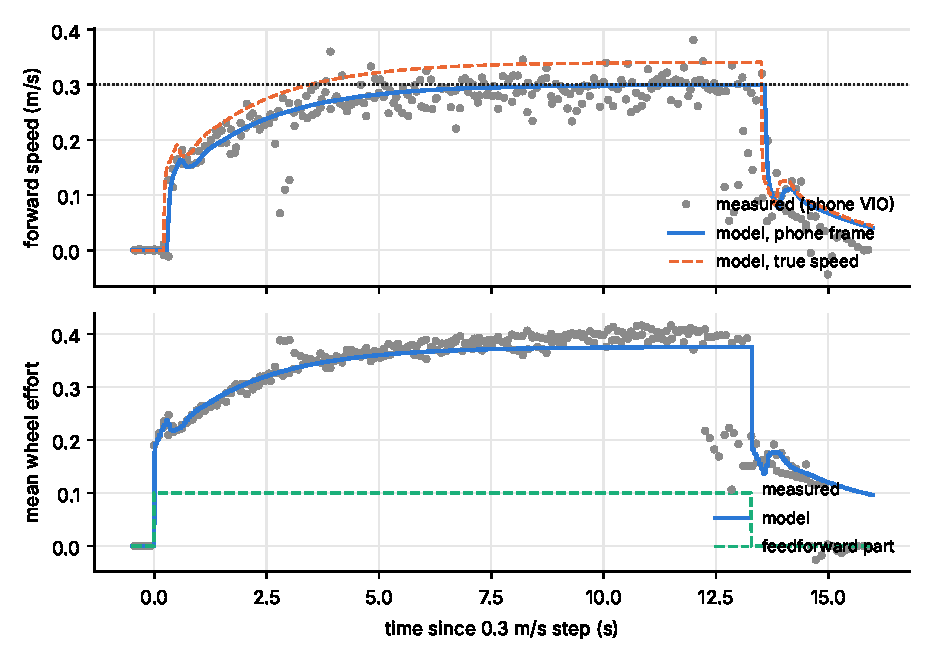
\includegraphics[width=0.85\textwidth]{figures/ctl_step_fit.pdf}
\caption{Two logged 0.3~m/s steps (grey) and the fitted model (blue). The effort first jumps to 0.19, the feedforward 0.1 plus the proportional term, and the integrator supplies the remaining 0.2 over about 4~s. After the target returns to zero the integrator still holds about 0.2 of effort, so the rover rolls on for about 1.3~s.}
\label{fig:stab-step}
\end{figure}

The controller's assumption, $K = 3$~m/s, is about 2.8 times the measured gain.
Its feedforward therefore supplies 0.1 of the 0.39 effort that 0.3~m/s needs, and the integrator supplies the rest.
That one mismatch explains the slow rise in Figure~\ref{fig:stab-step}, the 1.3~s roll-on after a stop, and, as the next section shows, the large stability margins.
Extrapolating the fitted line, full effort would give about $K(1 - d) \approx 1.0$~m/s; this lies beyond the measured range, and the ESC's mapping may not stay linear that far.

The deadband slows starts at low speed.
With $d = 0.06$, the first effort $k^{\text{ff}} v^\ast + k_p v^\ast$ is below the deadband for targets under about 0.1~m/s, and the rover waits for the integrator (Table~\ref{tab:stab-startup}).

\begin{table}[ht]
\centering
\caption{Simulated start-up of the as-built speed loop on the fitted plant.}
\label{tab:stab-startup}
\small
\begin{tabular}{@{}r r r@{}}
\toprule
Target (m/s) & First motion (s) & 90\% of target (s) \\
\midrule
0.05 & 1.52 & 5.8 \\
0.10 & 0.37 & 4.8 \\
0.20 & 0.22 & 4.2 \\
0.30 & 0.22 & 3.9 \\
\bottomrule
\end{tabular}
\end{table}

\section{Linear analysis of the speed loop}
\label{sec:stab-linear}

Away from the deadband and saturation, the speed loop is linear.
Feedforward is outside the loop and does not affect stability, so the loop transfer function is
\begin{equation}
  L(s) = \left(k_p + \frac{k_i}{s}\right) \frac{\kappa K\, e^{-\theta s}}{(\tau s + 1)(\tau_f s + 1)}, \qquad
  \theta = \theta_m + \theta_{\text{VIO}} + \tfrac{5}{2}T + \tfrac12 T,
  \label{eq:stab-loop}
\end{equation}
where $\kappa$ is the VIO scale, $T$ is the tick period, the zero-order holds of the 20~Hz motor write and the tick are approximated by half-period delays, and $\kappa K$ is the gain the phone sees.
At Release rates $\theta = 0.20 + 0.06 + 0.025 + 0.005 = 0.29$~s.

Two features of Equation~\eqref{eq:stab-loop} set its margins.
At low frequency the integrator dominates, and the loop crosses unity near $\omega_c \approx k_i \kappa K / \sqrt{1 - (k_p \kappa K)^2}$ while $k_p \kappa K < 1$.
At high frequency the PI term flattens to $k_p$ and the delay alone turns the phase, so the phase crosses $-180^\circ$ just below $\omega_{180} \approx \pi / \theta$ (the filter and motor lags pull it lower), independent of the gains, and the gain margin is close to
\begin{equation}
  \mathrm{GM} \approx \frac{1}{k_p \kappa K}.
  \label{eq:stab-gm}
\end{equation}
The proportional gain, not the integral gain and not the VIO latency, therefore decides how close the loop is to oscillation.

Table~\ref{tab:stab-margins} evaluates the loop for the as-built gains and for the variants that matter, and Figure~\ref{fig:stab-bode} shows the Bode plots.

\begin{table}[ht]
\centering
\caption{Margins of the speed loop. $\theta$ is the lumped loop delay; GM is at $f_{180}$. The as-built loop is in the first row.}
\label{tab:stab-margins}
\small
\begin{tabular}{@{}l r r r r r r r@{}}
\toprule
Case & $k_p \kappa K$ & $\theta$ (ms) & $f_c$ (Hz) & PM ($^\circ$) & DM (ms) & $f_{180}$ (Hz) & GM (dB) \\
\midrule
As built, Release, $\kappa = 0.88$ & 0.28 & 290 & 0.095 & 95 & 2790 & 1.37 & 11.1 \\
As built, Debug tick & 0.28 & 436 & 0.095 & 90 & 2640 & 0.92 & 10.6 \\
As built, $\kappa = 0.60$ & 0.19 & 290 & 0.063 & 93 & 4120 & 1.37 & 14.4 \\
As built, $\kappa = 1.00$ & 0.32 & 290 & 0.109 & 96 & 2440 & 1.37 & 10.0 \\
\midrule
Design assumption, $K = 3$ & 0.90 & 290 & 0.625 & 77 & 340 & 1.37 & 1.1 \\
Profile rule, $v_{\text{top}} = 1.0$ & 0.85 & 290 & 0.512 & 85 & 464 & 1.37 & 1.5 \\
Profile rule, Debug tick & 0.85 & 436 & 0.512 & 58 & 317 & 0.92 & 1.1 \\
\midrule
Matched feedforward only & 0.28 & 290 & 0.095 & 95 & 2790 & 1.37 & 11.1 \\
\bottomrule
\end{tabular}
\end{table}

\begin{figure}[ht]
\centering
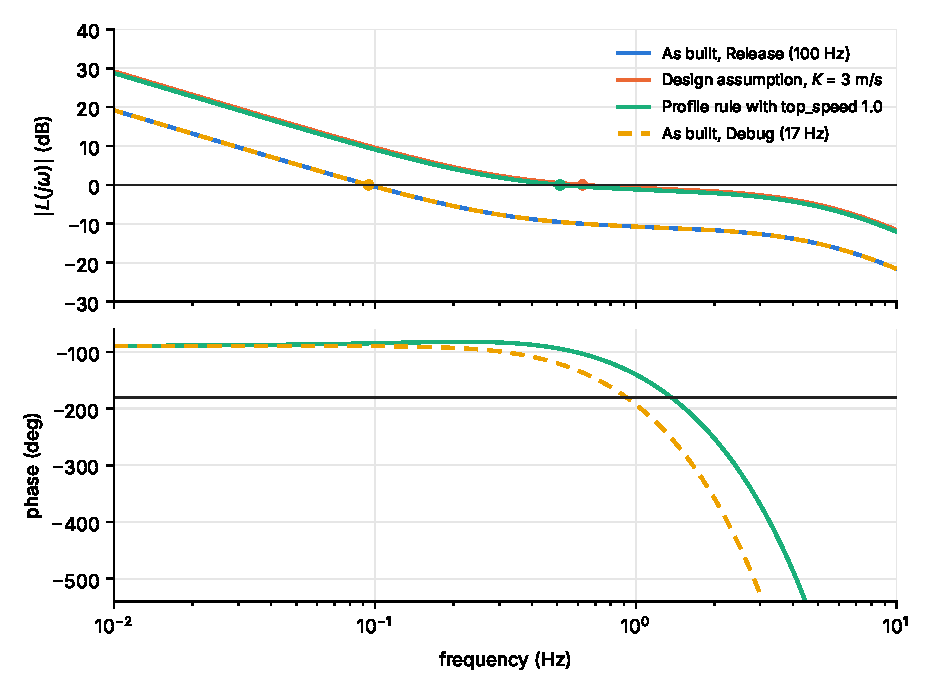
\includegraphics[width=0.85\textwidth]{figures/ctl_bode.pdf}
\caption{Bode plots of the speed loop. The as-built loop (blue, hidden under the dashed Debug curve in magnitude) crosses over at 0.095~Hz with 11~dB of gain margin. The loop the controller was designed for (orange) and the profile rule applied to the measured plant (green) cross over at 0.5--0.6~Hz with under 2~dB of gain margin. Dots mark the crossovers.}
\label{fig:stab-bode}
\end{figure}

Three readings follow from the table.

\paragraph{The as-built loop is stable for the wrong reason.}
It has very wide margins because the plant gain is a third of the design value.
Had Terra really reached 3~m/s at full effort, the same gains would leave 1.1~dB of gain margin: an increase in plant gain of 14\% would make it oscillate at about 1.4~Hz.

\paragraph{Correcting the profile is not enough.}
The rover profile derives all gains from the feedforward ($k_p = 0.9k^{\text{ff}}$, $k_i = 1.8k^{\text{ff}}$), so that each profile keeps ``the loop dynamics tuned on Terra'' (Section~\ref{sec:rover-profiles}).
That rule keeps $k_p K_{\text{assumed}} = 0.9$, which Equation~\eqref{eq:stab-gm} shows is too close to 1 for a loop with 0.29~s of delay.
Setting $v_{\text{top}}$ to the measured 1.0~m/s would raise $k_p$ to 0.9 and leave 1.5~dB of gain margin at Release rates and 1.1~dB in a Debug build.

\paragraph{The feedforward should be corrected on its own.}
Feedforward is outside the loop, so $k^{\text{ff}} = 1/(\kappa K) \approx 1.05$ with the as-built $k_p$ and $k_i$ keeps every margin in the first row, while the simulated 90\% rise time falls from 3.9~s to 0.36~s.
The integrator is then left to remove only the residual error and the deadband.
A safe rule for the profiles is to fix the feedforward from a measured top speed and to cap the proportional gain by the gain margin, $k_p \le 0.5/(\kappa K)$ for 6~dB, with $k_i \approx 2k_p$.

\section{Delay}
\label{sec:stab-delay}

Figure~\ref{fig:stab-delay} stacks the loop delay and compares it with the delay margins of Table~\ref{tab:stab-margins}.
The dead time between the effort leaving the phone and the wheels moving, 0.2~s from the fit, dominates.
It lumps the Bluetooth hop, the Pi relay, the ESC's response and the breakaway of a skid-steer chassis, and the step logs cannot separate them.
ARKit's 60~ms is the second item.
A Debug build adds 146~ms, because the motor write falls from every 50~ms to every 294~ms when the tick drops to 17~Hz.

\begin{figure}[ht]
\centering
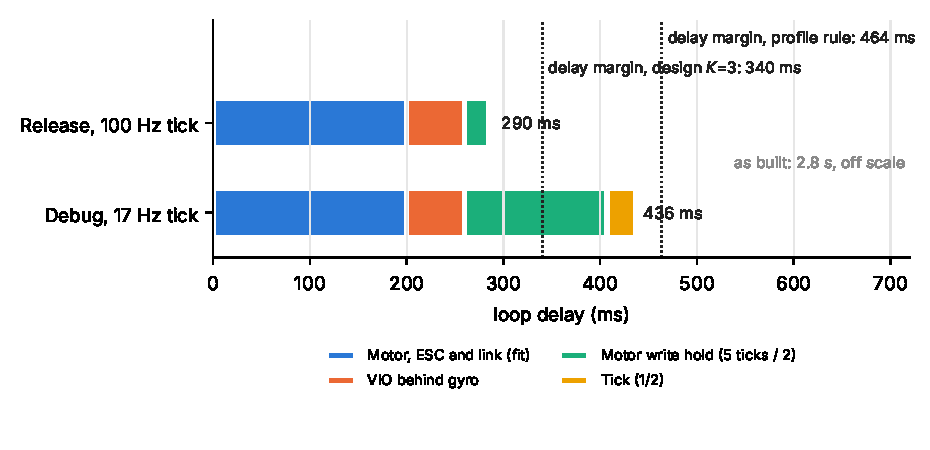
\includegraphics[width=0.9\textwidth]{figures/ctl_delay_budget.pdf}
\caption{Loop delay by source, Release and Debug, against the delay margin of the design gains and of the profile rule. The as-built delay margin, 2.8~s, is off the scale.}
\label{fig:stab-delay}
\end{figure}

Chapter~\ref{ch:phone} judged VIO latency against a budget of 382~ms (requirement R3).
That number is $(100^\circ - 45^\circ)/(360^\circ \times 0.4~\text{Hz})$: the delay that would use up 55$^\circ$ of phase at an assumed 0.4~Hz crossover.
The as-built loop crosses over at 0.095~Hz and has 2.8~s of delay margin, so R3 passes with far more room than stated.
The 382~ms figure is close to the right budget for the loop as designed (340~ms) and for a loop retuned by the profile rule (464~ms, 317~ms in Debug), and it should be read as the budget for a faster loop rather than for the current one.
In every case, the whole loop delay counts against the margin, not the VIO latency alone, and with the motor path at 0.2~s the phone's share is small.

\section{The VIO scale error}
\label{sec:stab-scale}

ARKit read distance and speed 8--19\% short in the motion-capture room (Section~\ref{sec:auto-state-validation}).
Inside the loop, a sensor scale $\kappa$ multiplies the loop gain.
Its effect on stability is small: over the measured range 0.60--1.00 the gain margin moves between 14.4 and 10.0~dB and the crossover between 0.063 and 0.109~Hz (Table~\ref{tab:stab-margins}).
Its effect on accuracy is direct.
The integrator drives the \emph{measured} speed to the target, so the true speed settles at $v^\ast/\kappa$: 0.34~m/s for a 0.30~m/s command at $\kappa = 0.88$, which matches the 0.31--0.34~m/s OptiTrack measured while the phone read 0.29--0.30, and 0.50~m/s at the outlier $\kappa = 0.60$.
Feedback cannot correct a sensor error; only a better scale estimate can (experiment E1b in Section~\ref{sec:phone-e1}).

\section{Saturation and anti-windup}
\label{sec:stab-saturation}

The controller has three saturating elements.
The common scale factor of Equation~\eqref{eq:mix} divides both wheels by the same number, so it preserves the turn ratio but cuts forward speed and yaw rate together.
The no-reverse rule zeroes a wheel that would counter-rotate, which on a turn at low speed is a one-sided saturation of the yaw effort.
And the integrators are clipped to $\pm 1$.

The back-calculation term limits the integrator while the output saturates.
In steady saturation $k_i e = k_{\text{aw}}(u - \bar u)$, so the unsaturated effort exceeds the applied effort by only $k_i e / k_{\text{aw}}$, 0.045 for a 0.3~m/s error, and the integrator stops near 0.86 instead of drifting to its clip.
The tracking time constant $1/k_{\text{aw}} = 0.25$~s is shorter than the 0.5~s integral time $k_p/k_i$ and much longer than the 10~ms tick, which is the usual choice~\citep{astrom2006advanced}.

Saturation matters for L3.
The pursuit law cruises at $v_c = 1.0$~m/s in the phone's frame, and the extrapolated top speed is about 0.9~m/s in that frame.
An L3 leg on open ground therefore asks for more than the rover can give: the effort sits at 1, the loop is open, and any turn command is scaled down with the forward command.
The planner and controller limits of 2~m/s are never reached.
\todo{Measure the top speed on CrabTrapBot with OptiTrack and set $v_c$ below it.}

\section{Deadband and limit cycles}
\label{sec:stab-deadband}

A deadband is a static nonlinearity with no memory, so its describing function~\citep{slotine1991applied} is real.
For a sinusoid of amplitude $A$ at its input, a deadband $d$ has gain $N(A) \in [0, 1)$, rising to 1 as $A$ grows.
A limit cycle needs $L(j\omega) = -1/N(A)$, and $-1/N(A)$ lies on the negative real axis to the left of $-1$.
A loop that is stable with unit gain never meets that ray, so \emph{an uncompensated deadband cannot make Terra's speed loop oscillate}.
It costs start-up time (Table~\ref{tab:stab-startup}) and, at very low targets, lets the integrator creep the wheel out of the deadband.

The compensation in Terra PR~\#71 changes this.
The lift $u' = \operatorname{sgn}(u)(d_c + (1 - d_c)|u|)$ adds a jump of $d_c$ at zero.
If the motor's true deadband $d_t$ equals $d_c$, the two cancel and the loop is linear.
If $d_c > d_t$, a relay of height $h = (d_c - d_t)/(1 - d_c)$ remains, whose describing function is $N(A) = 1 + 4h/(\pi A)$.
Now $-1/N(A)$ lies between $-1$ and 0, and it meets the Nyquist curve where the curve crosses the negative real axis, at $-1/\mathrm{GM}$.
The predicted limit cycle has the phase-crossover frequency $f_{180}$ and the effort amplitude
\begin{equation}
  A^\ast = \frac{4h}{\pi(\mathrm{GM} - 1)},
\end{equation}
and it is stable: smaller oscillations see a larger gain and grow, larger ones shrink.

Terra runs with $d_c = 0$ and is not affected.
terra-mini runs with $d_c = 0.3$, an estimate that has not been measured, and with the profile rule's gains ($k_p \kappa K = 0.79$, 2.2~dB of gain margin even with exact compensation).
Table~\ref{tab:stab-mini} and Figure~\ref{fig:stab-df} evaluate it with the same 0.2~s motor delay as Terra; terra-mini's plant has not been fitted, and its top speed of 0.8~m/s is the profile's estimate.

\begin{table}[ht]
\centering
\caption{terra-mini's speed loop at 0.1~m/s, by the motor's true deadband. Compensation is $d_c = 0.3$. Prediction by describing function; simulation of the ported controller.}
\label{tab:stab-mini}
\small
\begin{tabular}{@{}r r r r r r@{}}
\toprule
True $d_t$ & GM (dB) & Relay $h$ & Predicted $f$ (Hz) & Simulated $f$ (Hz) & Simulated speed, peak to peak \\
\midrule
0.3 & 2.2 & 0 & -- & -- & 0 (no cycle) \\
0.2 & 3.4 & 0.14 & 1.37 & 1.33 & 0.57~m/s \\
0.1 & 4.4 & 0.29 & 1.37 & 1.40 & 0.84~m/s \\
\bottomrule
\end{tabular}
\end{table}

\begin{figure}[ht]
\centering
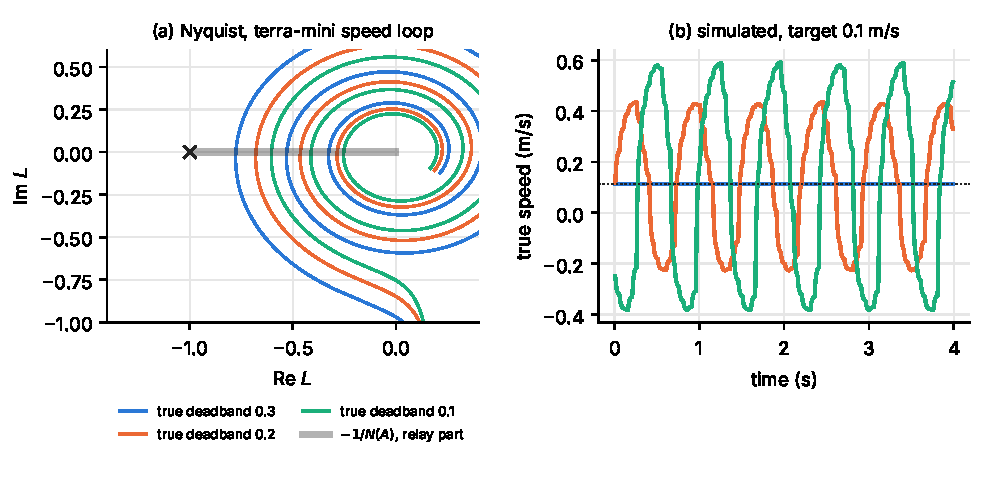
\includegraphics[width=0.95\textwidth]{figures/ctl_deadband_df.pdf}
\caption{(a) Nyquist curves of terra-mini's speed loop and the describing-function locus of an over-compensated deadband (grey). Each crossing of the negative real axis between $-1$ and 0 is a limit cycle. (b) The simulated limit cycles at a 0.1~m/s target: the wheels reverse every cycle.}
\label{fig:stab-df}
\end{figure}

The prediction and the simulation agree to within 3\% in frequency.
The amplitudes are large because the gain margin is small: with a margin of 3--4~dB, a relay of 0.14--0.29 is enough to swing the wheels through reverse at 1.4~Hz.
The safe direction for an unknown deadband is to under-compensate.
\todo{Measure terra-mini's deadband (slowest effort that turns each wheel on the floor) before setting $d_c$, and retune its $k_p$ by Equation~\eqref{eq:stab-gm}.}

\section{Safety holds and integrator windup}
\label{sec:stab-holds}

Section~\ref{sec:arch-timing} showed that most early faults were holds, not control-law faults.
The loop sees two kinds of hold, and they treat the integrators differently (Table~\ref{tab:stab-holds}).

\begin{table}[ht]
\centering
\caption{Hold types and what they do to the speed loop.}
\label{tab:stab-holds}
\small
\begin{tabularx}{\textwidth}{@{}>{\raggedright\arraybackslash}p{0.24\textwidth} >{\raggedright\arraybackslash}p{0.22\textwidth} X@{}}
\toprule
Hold & Integrator & Effect \\
\midrule
Controller hold: stale IMU ($\ge 0.5$~s) or VIO ($\ge 0.35$~s), stale target, step $> 0.1$~s, tracking lost; turning-limiter step $> 0.1$~s & Cleared & Bumpless but lossy. After release the effort restarts at $k^{\text{ff}}v^\ast + k_p e$ = 0.19 and the speed recovers over about 4~s. Repeated holds lower the mean speed. \\
Gate hold: phone mount not confirmed, Bluetooth link not ready, emergency stop latched & Keeps integrating & The controller still sees a fresh target and a still rover, so the integrator ramps at $k_i e$ = 0.18~s$^{-1}$ and parks at 0.86. On release, full effort drives the rover to about 1.0~m/s. \\
\bottomrule
\end{tabularx}
\end{table}

\paragraph{Gate holds wind the integrator up.}
In \texttt{drive\_loop.rs} the controller steps before the motor gate decides, and the gate's holds never reach the controller.
The journal of October 26 contains a 13~s run in which the mount check held the motors while a 0.3~m/s target was active.
The logged effort ramps from 0.19 to 1.0 in 4.5~s and stays there, exactly as the model predicts (Figure~\ref{fig:stab-holds}a).
That run ended with the target returning to zero, which resets the integrator.
Had the hold been released with the target still active, the model predicts a surge to 1.0~m/s within 0.5~s, three times the commanded speed, taking 6~s to settle (Figure~\ref{fig:stab-holds}b); in the first motion-capture session, run B\_v0.3\_r1 sat still for 10.7~s and then surged to about 0.7~m/s, which fits this mechanism but was not logged at the gate.
The fix is conditional integration: when the gate holds, freeze or clear the integrators exactly as a controller hold does.

\paragraph{Controller holds sap speed.}
Clearing the integrators is safe, but it throws away the 0.2 of effort that the integrator supplies at 0.3~m/s, and the loop needs about 4~s to rebuild it.
When holds repeat faster than that, the rover never reaches its target.
Table~\ref{tab:stab-periodic} simulates 150~ms holds at the period of the mesh walk that caused them in session 3 and at two other periods; Figure~\ref{fig:stab-holds}c shows the trace.
A 1.05~s period cuts the mean speed to 40\% of the target, which matches the session-3 runs that stopped short with the effort near 0.19 (Section~\ref{sec:arch-timing}).
With the feedforward matched to the plant (Section~\ref{sec:stab-linear}) the same holds would cost far less, because the restart effort would already be close to the steady effort.

\begin{table}[ht]
\centering
\caption{Mean true speed under periodic 150~ms controller holds, target 0.30~m/s (phone).}
\label{tab:stab-periodic}
\small
\begin{tabular}{@{}l r r@{}}
\toprule
Hold period & Mean true speed (m/s) & Fraction of no-hold speed \\
\midrule
None & 0.34 & 100\% \\
2.0~s & 0.18 & 52\% \\
1.05~s (session-3 mesh walk) & 0.14 & 40\% \\
0.5~s & 0.09 & 27\% \\
\bottomrule
\end{tabular}
\end{table}

\begin{figure}[ht]
\centering
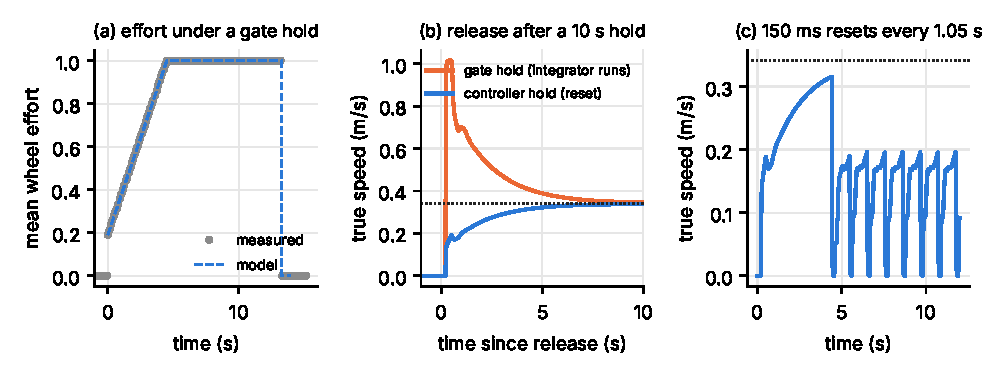
\includegraphics[width=\textwidth]{figures/ctl_holds.pdf}
\caption{(a) Logged effort during a mount-check gate hold (grey) and the model (dashed). (b) Simulated release after a 10~s hold: a gate hold (orange) surges to three times the target; a controller hold (blue) recovers slowly. (c) Simulated 150~ms controller holds every 1.05~s. Dotted lines: the true speed of a 0.30~m/s command.}
\label{fig:stab-holds}
\end{figure}

\section{Tick rate, jitter and sampling}
\label{sec:stab-tick}

At 100~Hz the controller samples 100 times faster than its 0.095~Hz crossover and 70 times faster than its 1.4~Hz phase crossover; the forward-Euler integrator and the half-period hold delay are negligible, and the continuous analysis above holds.
The slowest sampled element is the 20~Hz motor write, which Equation~\eqref{eq:stab-loop} already includes.

Tick rate matters through jitter rather than through sampling.
Three gates reject a long step: the controller's 0.1~s maximum step, the turning limiter's 0.1~s maximum step, and the IMU freshness gate.
Each turns a late tick into a controller hold, and so into the speed loss of Table~\ref{tab:stab-periodic}.
In the Debug run of October 27, with the control queue 60\% busy, 233 ticks would have seen an IMU older than 0.1~s; at the 0.5~s gate of Terra PR~\#92 only one would.
The Release runs had none at either threshold (Table~\ref{tab:phone-release}).
The 0.1~s step limits of the controller and the turning limiter remain, and they are the likely cause of the five straight runs that ended after about one second in the fourth motion-capture session.

One planner setting depends on the tick rate in a way the code does not state.
The local planner builds its velocity window as $\pm a\,\Delta t$ around the last command with $\Delta t$ fixed at the 0.1~s planner step, and the arbiter calls it on every 10~ms tick for managed commands, without the 0.1~s plan cache that unmanaged commands use.
Read from the code, the planner can therefore move the forward command by 0.1~m/s per tick, ten times the 1~m/s$^2$ it is configured for.
The turning limiter, which uses real timestamps, still bounds the yaw rate.
\todo{Confirm the effective linear acceleration of managed commands from a 100~Hz log.}

\section{The yaw-rate loop}
\label{sec:stab-yaw}

The yaw loop has the same structure as the speed loop, closed on the gyro, which has no VIO lag, so its delay is 0.23~s.
Its plant gain $K_\psi$ (rad/s per unit of differential effort) has not been measured: the arcs of October 26 were run before Terra PR~\#74, when the estimator read the phone's roll rate as yaw rate, and the logged yaw loop chased that wrong signal through $\pm 2$~rad/s swings.
The design value implied by the feedforward is $K_\psi = 1/k^{\text{ff}}_\omega = 5$~rad/s.
If the yaw path is over-estimated by the same factor as the forward path, $K_\psi \approx 1.6$--1.8.
Table~\ref{tab:stab-yaw} gives both ends.

\begin{table}[ht]
\centering
\caption{Margins of the yaw-rate loop and of the L3 heading loop closed around it ($k_\theta = 1.6$~s$^{-1}$), for the two plausible yaw plant gains.}
\label{tab:stab-yaw}
\small
\begin{tabular}{@{}l r r r r@{}}
\toprule
& \multicolumn{2}{c}{$K_\psi = 1.6$~rad/s} & \multicolumn{2}{c}{$K_\psi = 5$~rad/s (design)} \\
\cmidrule(lr){2-3}\cmidrule(lr){4-5}
& Yaw rate & Heading & Yaw rate & Heading \\
\midrule
Crossover (rad/s) & 0.49 & 0.96 & 1.73 & 1.90 \\
Phase margin ($^\circ$) & 92 & 57 & 95 & 76 \\
Gain margin (dB) & 15.9 & 17.7 & 6.0 & 7.8 \\
Delay margin (ms) & 3310 & 1040 & 960 & 700 \\
\bottomrule
\end{tabular}
\end{table}

Either way the yaw loop is stable.
At the design gain its gain margin, 6~dB, is the smallest of Terra's loops, and a yaw plant faster than designed, for example on a low-friction floor where the skid factor falls, would erode it.
\todo{Measure $K_\psi$ from 100~Hz logs of arcs after Terra PR~\#74 with the landscape roll set (experiment E1c).}

\section{L3 path following}
\label{sec:stab-l3}

\subsection{Heading loop}

Near alignment the pursuit law is a proportional heading loop around the yaw-rate loop: with the yaw loop's closed-loop response $T_\omega(s)$ from reference to yaw rate, feedforward included,
\begin{equation}
  L_\theta(s) = \frac{k_\theta\, T_\omega(s)}{s}.
\end{equation}
Table~\ref{tab:stab-yaw} gives its margins: 57--76$^\circ$ of phase margin and 0.7--1.0~s of delay margin.
The heading loop crosses over at about the same frequency as the yaw loop beneath it, so the two are not separated in time scale; the yaw feedforward is what keeps $T_\omega$ close to 1 at the heading crossover ($|T_\omega| = 0.75$--1.0 at 0.5~rad/s).

The linear picture omits the turning limiter, whose yaw-rate cap $|v|/R_{\min}$ and 0.5~rad/s$^2$ slew are active in every L3 turn.
Figure~\ref{fig:stab-l3}a simulates a 0.5~rad bearing step through the full chain (pursuit law, limiter, both PI loops, fitted forward plant, unicycle).
The limiter slows the response but does not destabilise it: overshoot stays under 4$^\circ$ in every case, and settling to within 3$^\circ$ takes 1.8--6.1~s (Table~\ref{tab:stab-l3}).
The slowest case is a slow cruise, because the cap ties the turn rate to the forward speed.

\begin{table}[ht]
\centering
\caption{Simulated response to a 0.5~rad bearing step at L3.}
\label{tab:stab-l3}
\small
\begin{tabular}{@{}r r l r r r@{}}
\toprule
$K_\psi$ & Cruise (m/s) & Limiter & Overshoot ($^\circ$) & Settling to 3$^\circ$ (s) & Peak yaw rate (rad/s) \\
\midrule
1.6 & 0.3 & on & 3.1 & 6.1 & 0.24 \\
1.6 & 1.0 & on & 3.8 & 4.9 & 0.32 \\
1.6 & 1.0 & off & 2.9 & 2.0 & 0.31 \\
5.0 & 1.0 & on & 0.0 & 1.8 & 0.58 \\
\bottomrule
\end{tabular}
\end{table}

\begin{figure}[ht]
\centering
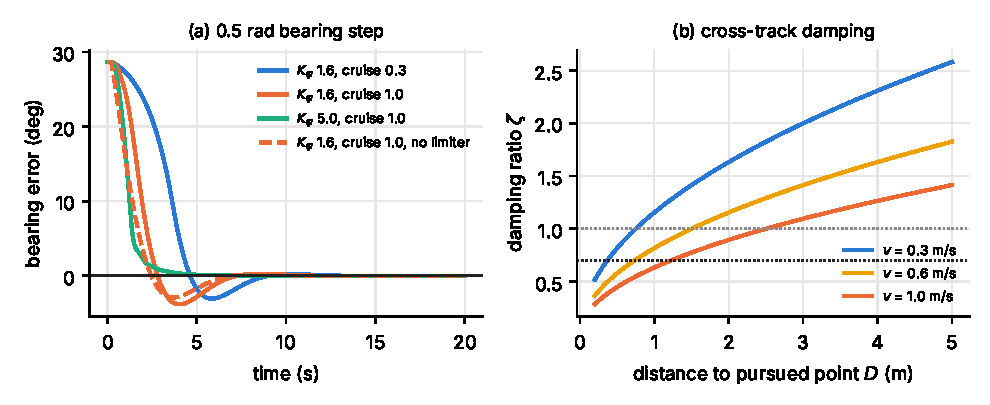
\includegraphics[width=\textwidth]{figures/ctl_l3.pdf}
\caption{(a) Bearing error after a 0.5~rad step, full nonlinear chain. (b) Cross-track damping ratio of the pursuit law, Equation~\eqref{eq:stab-zeta}; dotted lines at 0.7 and 1.}
\label{fig:stab-l3}
\end{figure}

\subsection{Cross-track dynamics}

L3 pursues the farthest route point still in line of sight, at distance $D$.
For a small lateral offset $y$ from the line to that point and a small heading $\psi$ relative to it, the bearing error is $-(y/D + \psi)$, so with an ideal inner loop
\begin{equation}
  \dot y = v\psi, \quad \dot\psi = -k_\theta\left(\psi + \frac{y}{D}\right)
  \;\Rightarrow\;
  \ddot y + k_\theta \dot y + \frac{k_\theta v}{D} y = 0, \qquad
  \zeta = \frac12\sqrt{\frac{k_\theta D}{v}}.
  \label{eq:stab-zeta}
\end{equation}
This is the usual look-ahead trade of pure pursuit~\citep{coulter1992pursuit}: a far point damps and a near one oscillates.
At $v = 1$~m/s, $\zeta$ falls below 0.7 when $D < 1.2$~m and below 0.5 when $D < 0.6$~m (Figure~\ref{fig:stab-l3}b).
Route corners are dropped at 0.2~m, and a corner whose successor is hidden is pursued down to that distance, so the last metre before such a corner is lightly damped.
At 0.3~m/s the same $\zeta$ needs only a third of the distance.

\subsection{The heading gate}

The pursuit law sets the forward speed to zero when the bearing error reaches $\gamma = 0.55$~rad.
On Terra, where turning in place is not allowed, the turning limiter's cap $|v|/R_{\min}$ is then zero as well, so the rover can neither drive nor turn.
This is a structural dead zone, not an instability: any bearing change larger than 31$^\circ$, for example at a corner revealed late, stops the pursuit law, and the arbiter's multi-point manoeuvre (Section~\ref{sec:auto-turning}) has to take over.
terra-mini, which may spin, does not have this dead zone.

\section{Summary and recommendations}
\label{sec:stab-summary}

Table~\ref{tab:stab-recs} collects what the analysis recommends and what it still needs.

\begin{table}[ht]
\centering
\caption{Recommendations from this chapter.}
\label{tab:stab-recs}
\small
\begin{tabularx}{\textwidth}{@{}>{\raggedright\arraybackslash}p{0.30\textwidth} >{\raggedright\arraybackslash}p{0.25\textwidth} X@{}}
\toprule
Finding & Evidence & Action \\
\midrule
Feedforward assumes 3~m/s; plant gives about 1.0 & Fit, Table~\ref{tab:stab-plant} & Set Terra's feedforward from a measured top speed; keep $k_p$, $k_i$ (rise 3.9~s $\to$ 0.36~s, same margins). \\
Profile rule ties $k_p$ to feedforward & Table~\ref{tab:stab-margins} & Cap $k_p \le 0.5/(\kappa K)$ for 6~dB gain margin; $k_i \approx 2k_p$. \\
Gate holds wind up the integrator & Logged ramp, Figure~\ref{fig:stab-holds}a & Freeze or clear the integrators whenever the motor gate holds. \\
Controller holds cost speed & Table~\ref{tab:stab-periodic}, session 3 & Keep holds rare (Release builds, work off the control queue); matched feedforward lowers the cost. \\
VIO scale error & Table~\ref{tab:vio-scale} & Not a stability issue; correct the scale (E1b). \\
terra-mini deadband unmeasured & Table~\ref{tab:stab-mini} & Measure it; under-compensate when unsure. \\
L3 cruise above top speed & Section~\ref{sec:stab-saturation} & Set $v_c$ below the measured top speed. \\
Planner window assumes a 10~Hz call & Code reading & Use the real tick interval for the window. \\
\bottomrule
\end{tabularx}
\end{table}

The analysis rests on a plant fitted from two steps at one speed, logged at 10~Hz.
The next measurements, in order of what they would change, are: speed steps at 0.1, 0.3 and 0.6~m/s with OptiTrack and 100~Hz phone logging, to fit $K$, $d$, $\tau$ and $\theta_m$ properly and check linearity; the same for arcs, to measure $K_\psi$; and a gate-hold release test before and after the integrator fix, to confirm the surge and its removal.
\todo{Run the plant-identification steps and replace the fitted values in Table~\ref{tab:stab-plant}.}
